
\chapter{Methods}
\label{chapter:methods}
% this should be for general methods 
% within each chapter I can talk about how I used these methods

In this chapter I discuss computational methods that I used throughout my PhD. 
Chief among them is the RNA-seq analysis pipeline. 
My project has mostly consisted of processing very large amounts of RNA-seq data and has required a stable, modular and workflow that can be run in parallel across multiple computers.
I will describe each step of the pipeline in detail.
I then go on to discuss tools for analysing differential gene expression and particularly differential splicing.
These tools provide lists of genes and splicing events but do not by themselves provide biological insight.
It is important to use other sources for data to put these results in a functional context. 
I describe methods for using RNA-protein interaction data, motif searching, sequence conservation and gene ontology.

\section{Library preparation and sequencing}
I feel it is important to understand the preparation of a short read sequencing library so as to best interpret the data in downstream analyses. 
Before sequencing can take place, important decisions must be made about the how the sequencing will be done as this is crucial for what questions can be asked. 

\subsection{Considerations when preparing an RNA sequencing library}

% Total RNA vs PolyA
RNA sequencing libraries are created either from polyadenylated RNA (polyA+) or from total cellular RNA (total RNA).
Total RNA libraries must be depleted of ribosomal RNA species, which consist of 80-90\% of all RNA species in the cell \citep{Wilhelm2009}. % reference?
RIbosomal depletion is performed using biotinylated probes that hybridise to ribosomal RNA transcripts. The most popular kit for this is the Ribo-Zero method (Illumina).
In contrast, polyA+ libraries are created  by RNA extraction with oligo d(T) beads, which should hybridize to polyadenylated RNA only. 
This is sometimes referred to a mRNA-seq, but as multiple non-coding RNAs are polyadenylated this is a misnomer.

Choosing between the two library preparation methods depends both on the biological question of interest but also on the quality of the RNA to be sequenced.
polyA+ RNA-seq has a coverage bias towards the 3' end of transcripts and this is exacerbated when RNA is highly fragmented.  
Total RNA in contrast has a much more even coverage throughout the body of each transcript.
For post-mortem tissue samples, total RNA is usually preferred due to the high RNA degradation which can be caused by changes in tissue pH or through tissue fixation with formalin.

When quantifying gene expression, total RNA and polyA+ sequencing libraries are highly concordant \citep{Cui2010,Zhao2018}. 
The effect of 3' bias can be ameliorated by focusing analysis on the 3' end of transcripts where coverage will be highest. 
%polyA+ libraries made from degraded RNA or certain library preparation kits tend to be highly biased towards coverage towards the 3' end of genes which can confound analyses.
When investigating splicing, total RNA libraries will contain higher proportions of intronic reads, originating from unspliced nascent RNA \citep{Ameur2011}.
This can confound analysis. 
For investigating small RNA species such as small nucleolar RNAs and microRNAs, a size fractionation is done to enrich the sample for these small species which are relatively less abundant than mRNA .

For the sequencing itself, there are 4 key considerations: the number of reads sequenced per sample, the length of the reads, whether single- or paired-end sequencing will be done, and whether the library will be stranded.
Single- and paired-end sequencing refers to whether one end of the cDNA fragment or both ends will be sequenced.
Stranded libraries retain the direction of transcription for each RNA fragment. 
This allows for the discovery of antisense transcripts, such as promoter antisense and 3' antisense transcripts, which are ubiquitious in eukaryotes but poorly understood \citep{Lavorgna2004}.
This also improves quantification of transcripts from genes that run into each other from opposing ends. 

These 4 parameters affect the types of analyses that can be performed with the sequencing data.
They also substantially influence the cost of the experiment.
For a given number of sequencing reads 25 base pair unstranded single end sequencing is far cheaper than 300bp stranded paired end, the current maximum with Illumina technology. 

The first outcome is alignment rate - the proportion of sequencing reads that uniquely map to the genome of interest. 
Here, longer reads increase the unique alignment rate, as does paired end versus single end due to the added constraint on alignment given by both reads in the pair. 
For detecting lowly expressed transcripts, sequencing depth is crucial. 
For splicing analysis, the most important metric is the number of read that span splice junctions. Most splicing software relies on these unction reads.
With longer reads, the chances of any given read overlapping an intron increase so long (>=100bp) reads are highly recommended.
A study compared RNA-seq samples at different simulated read lengths either paired or single ended.
The authors recommended 50bp single end minimum for differential gene expression and 100bp paired end for splicing \citep{Chhangawala2015}. 


\begin{figure}[h!]
	\begin{center}
		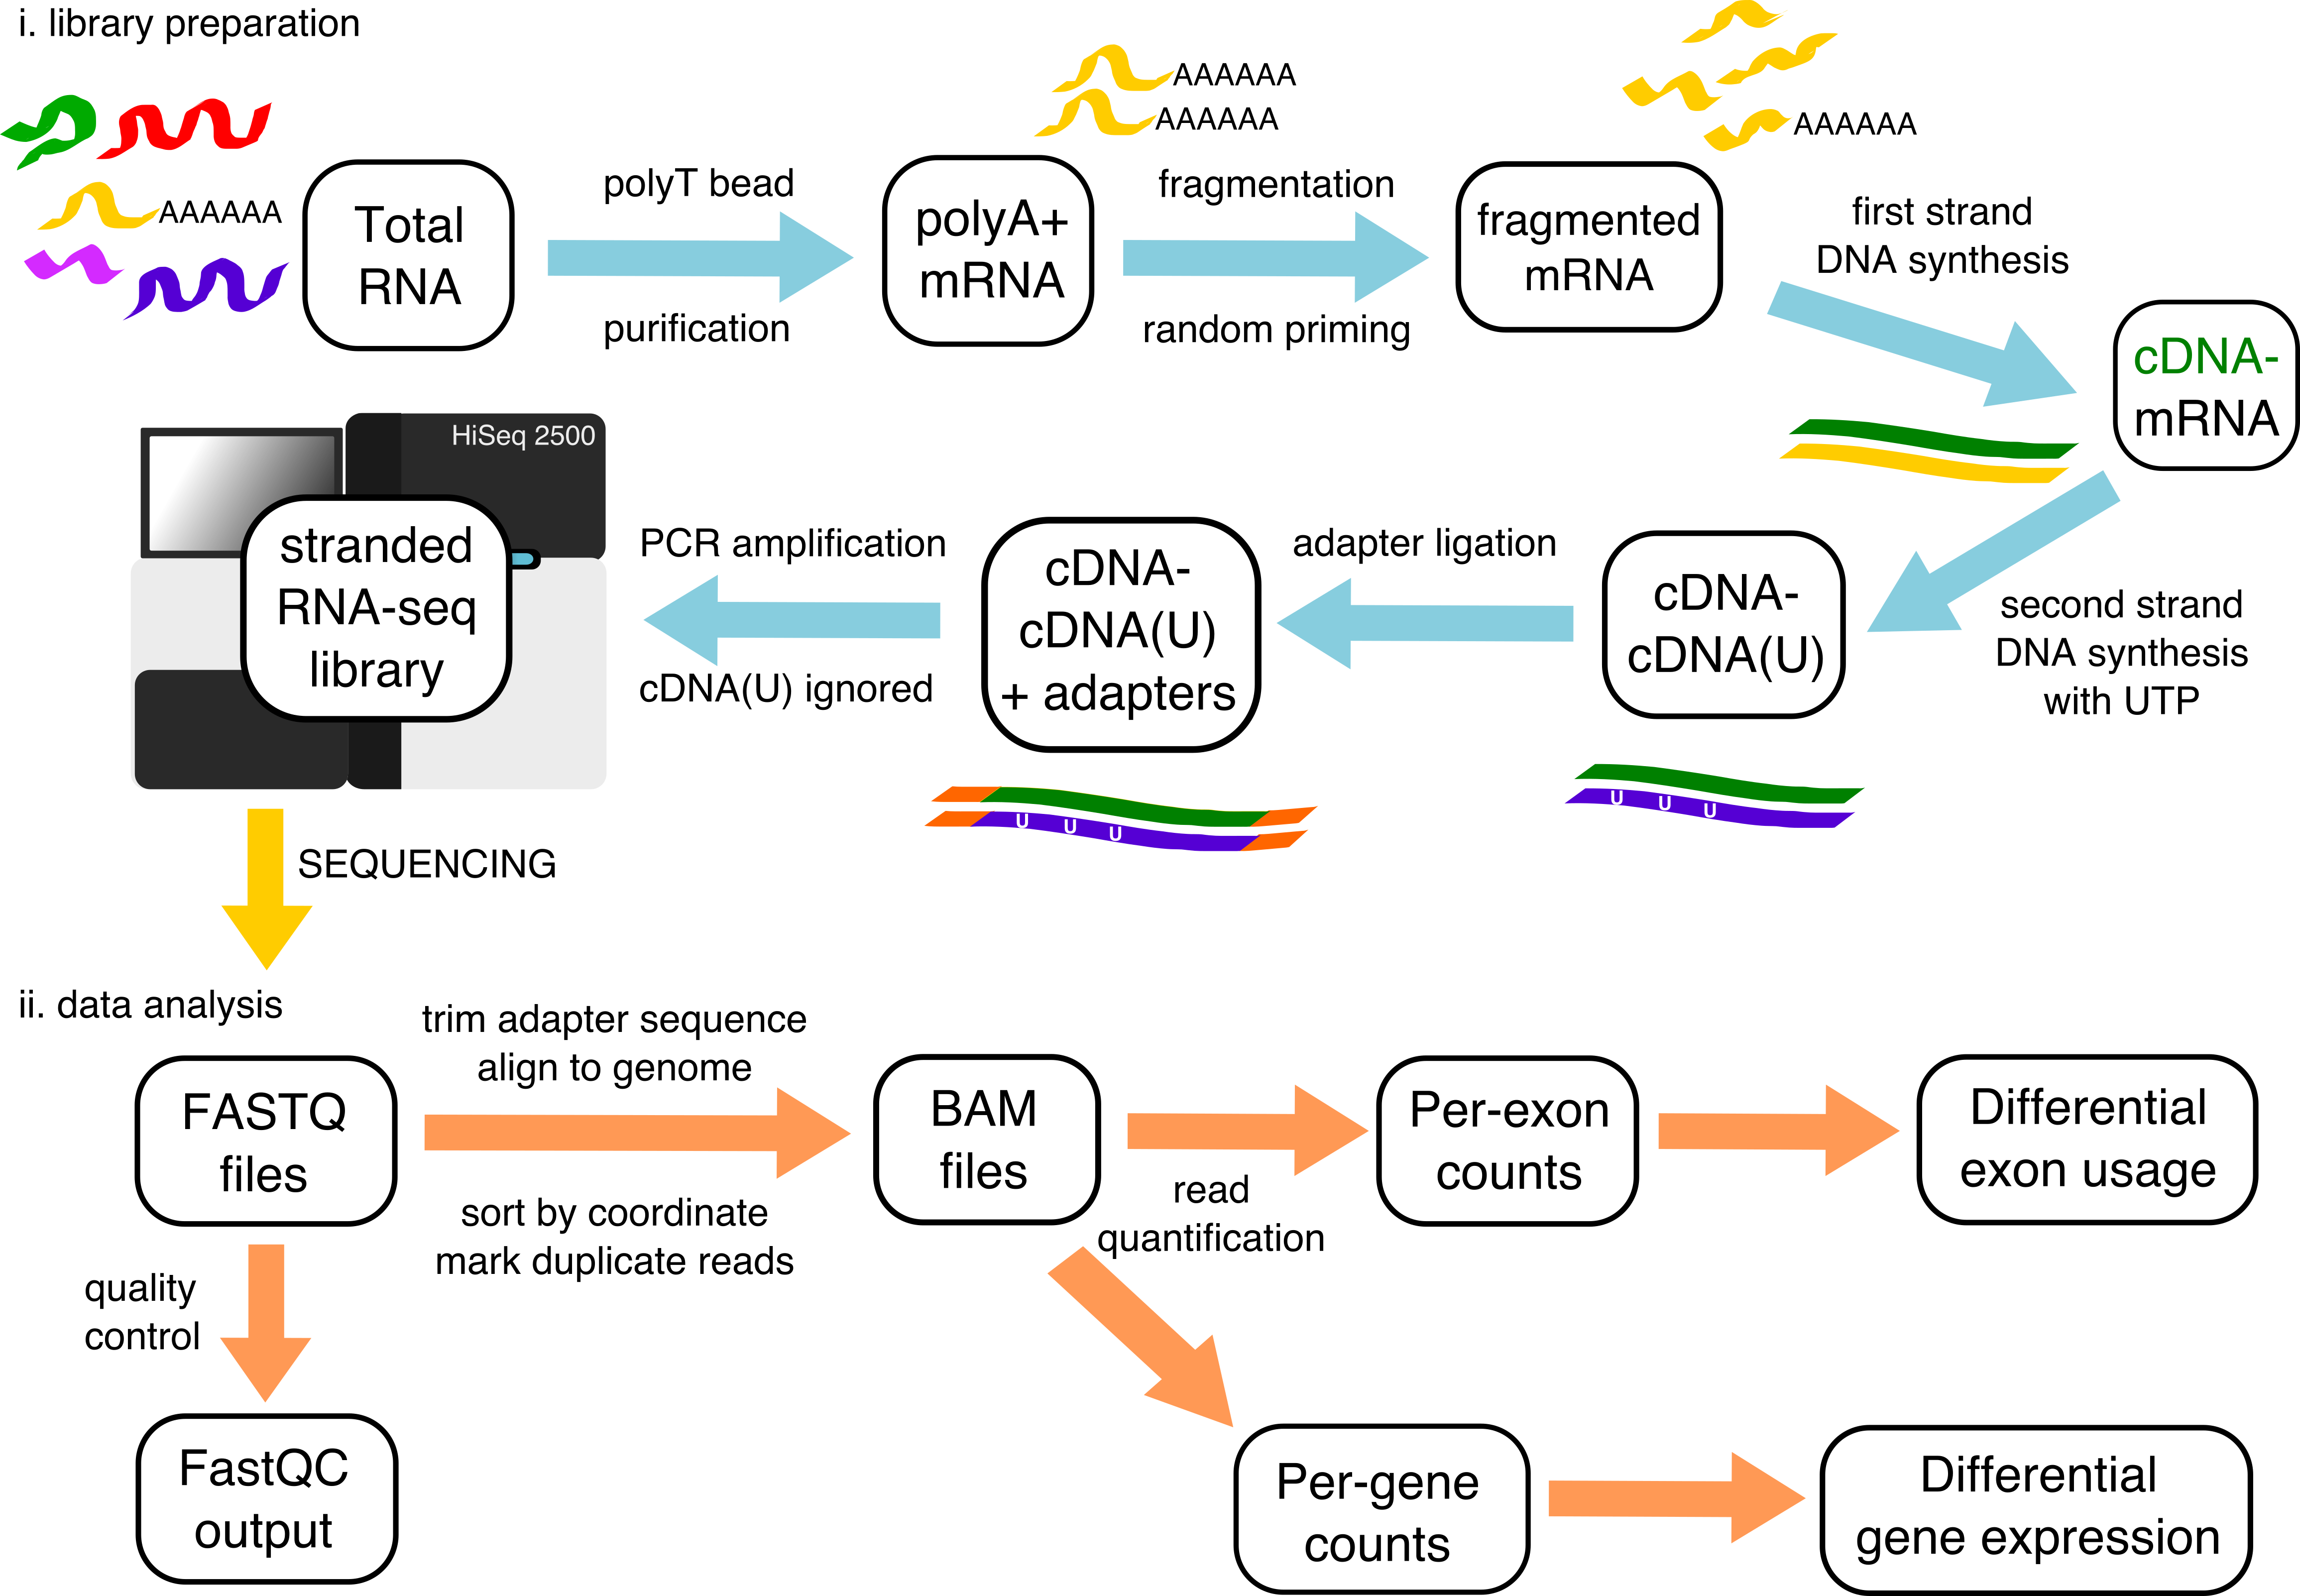
\includegraphics[width=14cm]{Figures/02_methods/RNAseq_pipeline_schematic.png}
	\end{center}
	\caption{Pipeline for stranded RNA-seq preparation and analysis}
	i) Library preparation from total RNA extraction and strand-specific amplification\\
	ii) Bioinformatic analysis workflow to align reads and test for differential gene expression and exon usage
\end{figure}

\subsection{Sequencing library preparation}

The description below is of a polyA+ enriched  stranded RNA-seq library preparation for Illumina sequencing.
Total RNA is extracted from cells or tissues using Trizol or a similar phenol/chloroform reagent \citep{Chomczynski1987}. The majority of RNA species in the cell are ribosomal RNAs. 
To enrich for mRNA species the RNA is mixed with magnetic beads that are bound to poly(Thymine) oligonucleotides, complementary to the poly(Adenine) tail at the 3' end of mRNA. 
The RNA is then fragmented. 
As paired-end sequencing extracts information from each end of the fragment it is important to consider the fragment size in light of the subsequent length of the reads, as with short fragments and long reads the read pairs will overlap leading to redundant information. 
Pseudo-random barcodes are ligated to each fragment to allow for reverse transcription. 
This pseudo-randomness does cause bias towards particular sequences % CITE
The first round of reverse-transcription is carried out forming double stranded DNA-RNA hybrids. 
These complexes are annealed and a second reverse-transcription reaction is carried out in the presence of Uracil instead of Thymine, creating double stranded DNA. The Uracilated DNA strand is now in the same orientation as the original mRNA fragment. 
Polymerase chain reaction amplification is then carried out where the uracil containing DNA and the RNA are ignored by the polymerase. 
The resulting library is strand-specific as all the DNA fragments are antisense to the original RNA fragments. Further adapters are added for sequencing in the flowcell and to give the fragments from each sample an identifier as multiple samples are usually pooled together. 
The standard Illumina paired-end sequencing reaction ligates the amplified fragments to wells in the flowcell which then form clusters of identical amplified fragments. Sequencing then occurs by sequential addition of fluorescent nucleotides along the length of a fragment in both directions, the  colour of which is recorded by a high resolution sensor. 
The identity of each nucleotide is determined and given a quality score based on the confidence of the measurement. 
The reads are converted from the basecall (BCL) format to a FASTQ file by the sequencing centre.
The FASTQ file specification \citep{Cock2009} encodes the unique read ID, the read sequence and a quality score. In paired end sequencing, reads of each pair share a read ID . 
Forward and reverse reads are written into separate files.  
The FASTQ file can be thought of as a digital encoding of the sequence of both ends of each cDNA fragment.


\section{The Plagnol lab RNA-seq pipeline}

A pipeline connects together multiple software tools to convert raw data into summaries and statistics.
The RNA-seq pipeline converts raw sequencing reads into counts of genes, exons and splice junctions for use in downstream analyses.
This was collaboratively developed by the group of Vincent Plagnol but adapted and occasionally broken by myself
The pipeline is optimised for the UCL Computer Science cluster but is freely available to all from \url{github.com/plagnollab/RNASeq_pipeline/}.
The pipeline itself is written in the Bash programming language \url{http://www.gnu.org/software/bash/}. 
Individual modules for differential expression and splicing are written in the R statistical programming language \citep{Gentleman1996}. 

% snakemake and nextflow - better organised, more modular, help with cluster difficulties
The pipeline has been optimised for the UCL Computer Science cluster.
The cluster is made up of hundreds of individual computers (nodes), controlled from a head computer using the Sun Grid Engine system (Univa) for organising and distributing computational work.
This allows for individual steps of the pipeline to be run in parallel or series and link the completion of one step with the commencement of the next.
This makes running the pipeline from start to finish automatic and as fast and efficient as possible.
However, I have encountered numerous problems while doing my research due to instability and breakages of individual nodes in the cluster.
This can be ameliorated by using cluster-aware pipeline frameworks such as SnakeMake or NextFlow \citep{Koster2012,DiTommaso2017}. 
These frameworks can restart computation when a particular node fails, and increase hardware requirements when particular steps fail.
I hope that the next version of the pipeline will be written using one of these frameworks.


\subsection{Quality control and read alignment}

% mention multiQC
% talk about QC steps - GC content, random hexamer bias, 3' bias

The first step in any analysis is quality control of the FASTQ files. 
Popular tools like \textit{FastQC} (\url{bioinformatics.babraham.ac.uk/projects/fastqc/}) analyse a set of FASTQ files and produce visualisations of multiple diagnostic tests. 
It can be useful to observe the range of quality scores and how they alter throughout the length of a read to diagnose faults during the sequencing reaction. 
Another important diagnostic is the presence of adapter sequences within reads. 
This can occur when the fragmentation step is too aggressive or when the original RNA sample is heavily degraded, often the case in human post-mortem tissue samples. 
With very short fragments, the sequential addition of nucleotides runs into the adapter sequence of the reads, making these reads much more difficult to align. 
These universal adapter sequences can be removed by software such as \textit{Trim Galore!} (\url{bioinformatics.babraham.ac.uk/projects/trim_galore/}).
This can also remove low quality sequence from the ends of reads, which often occurs towards the end of an Illumina sequencing run. 

Following trimming, the FASTQ files must then be aligned to the genome of the species of interest. 
There have been great advancements in speed and accuracy in alignment algorithms, but the key difference between DNA and RNA alignment is the need for read splitting. 
As most mRNAs are spliced, any RNA fragment that originates from the boundary between two exons will need to be split and both pieces separately aligned to the genome. 
The interval between two pieces is then recorded by the aligner as a splice junction, the demarcation of where an intron was excised. 
The current state-of-the-art algorithm in both speed and accuracy at resolving splice junctions is \textit{STAR} \citep{Dobin2013-ra}.
\textit{STAR} derives its speed from loading the entire genome into memory and then mapping millions of reads per hour using a seed-and-extend algorithm, where small pieces of each read are aligned and incrementally extended to find the best possible split alignment. 
The alignment information for each read is recorded in a BAM file \citep{Li2009-hm}. 
Reads from each pair are initially recorded next to each other and the BAM file is ordered by the read name. 
However for most downstream analyses the BAM file must be re-ordered by genomic position. 
The pipeline does this using the \textit{Novosort} algorithm (\url{http://www.novocraft.com/products/novosort/}). 

Another potential issue in RNA-seq data, particularly in older data or from human brain-derived RNA, is a bias towards fragments from the 3' end of mRNAs. 
This can also occur due to mRNA degradation before the poly(Thymine) purification which will then bias the library to sequences closest to the bound polyadenylation site at the 3' end. 
This can be obvious when observing coverage across all genes with a diagnostic package such as \textit{QoRTS} or RNASeQC \citep{Hartley2015a, Deluca2012}. 
As most differential expression software assumes even coverage throughout a gene body, heavily degraded samples can skew the estimates of gene or exon expression.

For downstream expression analysis, the aligned reads are then quantified for a set of features. These features can either can be whole genes or individual exons. 
There are multiple annotations for the human and mouse genome for where the known genes and exons are but our pipeline uses the Ensembl transcript annotation as our reference \citep{Cunningham2015}. 
Reads that overlap each gene or individual exon are counted using \textit{HTSeq} \citep{Anders2015-wz}.

\subsection{Differential gene expression}

The most common application of RNA-seq is for an experiment comparing the abundances of different RNAs between conditions.
This could be for example between the knockdown of a particular gene and a control, or between a group of disease patients and a group of healthy controls. 
These experiments should be made up of multiple biological replicates, where RNA libraries have been prepared from different organisms or cell culture samples under the same conditions. 
This is so a fair assessment can be made of the biological variation in RNA abundance within each condition. 
This is in comparison to technical replicates, where the same library is sequenced multiple times, which only tell you about the variance between repeated measurements.
As the concordance between technical RNA-seq replicates is very high \citep{Mortazavi2008}, these are generally shunned in favour of biological replicates. 
RNA-seq is still an expensive experiment and the high cost limits a lab to sequence only a small number of biological replicates.
This limits the statistical power to detect small variations in RNA abundances and the confidence in the truth of one's results. 
There are multiple algorithms to test for differential expression but we settled on using the \textit{DESeq2} package for its statistical robustness and speed \citep{Love2014}. 
It is desiged to compensate for the small sample sizes used in a typical RNA-seq experiment, usually less than 5 per condition.

\textit{DESeq2} makes use of the fact that each sequencing library measures the abundance of tens of thousands of transcripts. 
The number of reads generated by each library can be highly variable and so this is also accounted for. 
\textit{DESeq2} normalises the read counts for each gene in each sample by the size of each sample's library, the \textit{size factor}. 
It then assumes that the normalised read counts fit a negative binomial probability distribution. 
It estimates the variance or dispersion in read count for each gene across all samples. 
To compensate for small sample sizes, which give a very high estimate of dispersion, it compares the dispersion between all genes and shrinks the estimate to a local average dispersion based on genes expressed at a similar level. 
Using these shrunken dispersion estimates, the software then fits two generalised linear models: a null model where condition has no effect and an alternative model where the change in condition explains the change in gene expression. 
The two models are compared with a Wald test on which model fits the data better, computing a P-value. 
The P-values generated for each gene are adjusted to correct for multiple testing using the Benjamini-Hochberg procedure \citep{Benjamini1995}. 
The output of a differential expression analysis gives both an adjusted P value for each gene and a fitted $log_2$ of the fold change in expression between the two conditions. 
This give you an estimate of the effect size. 
Fold-changes on the $log_2$ scale have the useful aesthetic property of being symmetrical around positive and negative powers of two.
Therefore a doubling of expression will have a $log_2$ fold change of $1$, and a halving will have a $log_2$ fold change of $-1$.


\section{Differential splicing}

Differential splicing is an analysis that looks for changes in splicing between conditions. 
How this is done depends on the frame of reference used. 
I will discuss examples of different approaches to differential splicing.

Methods for differential splicing have generally followed the progress of sequencing technology and cost. 
Advances in read length and depth of sequencing have driven the development of new algorithms that make use of the increasing availability of splice junction reads within samples.

I can group software packages into one of four categories based on what they consider to be the fundamental unit of differential splicing. 
All of these modern algorithms work best with high depth paired end data. The approaches based on junction reads also require long reads to maximise the information available.

\subsection{Exon quantifiers}
This tests for differences in the usage (read count) of a particular exon as a ratio of reads in all exons. This "corrects" for differences in baseline gene expression.  This approach was first used in the \textit{DEXSeq} package \citep{Anders2012}. 
\textit{DEXSeq} requires a flattened list of "union exons" which is a set of non-overlapping intervals for each exon from each annotated transcript in a given gene. 
RNA-seq seq reads can then be counted at each union exon. 
\textit{DEXSeq} normalises the per-exon counts to a library \textit{size factor} and compares the  normalised counts from each exon with the counts from all the exons in a gene.
It then fits a generalised linear model to compare the ratio of exon usage between biological conditions and estimates a fold-change, which is shrunken with a Bayesian shrinkage procedure.
The output of a \textit{DEXSeq} analysis is each union exon in a gene is given a $log_2$ fold change between conditions and an adjusted P value from the test. 
Although this can be used to demonstrate whether differential exon usage occurs due to a condition, it is inherently difficult to extract meaningful information about the underlying biology. 
A significant union exon may not correspond to real exon. Therefore, hits from \textit{DEXSeq} need to be closely analysed in the context of the gene they reside in. 
This approach is dependent on transcript annotation. 
DEXSeq has also been used to measure differential intron usage \citep{Li2015a}. This directly inspired my work on \textit{Cryptex}, a software pipeline for using splice junction reads to find novel exons which I discuss in \autoref{chapter:cryptic_exons}.
% rewrite
These algorithms are typified by the \textit{DEXSeq} approach \citep{Anders2012}, where the transcripts are flattened to create a set of unique exon "bins".  As the bins themselves may not actually be an exon it makes the results difficult to interpret, although this has been lessened in a new software package called \textit{JunctionSeq} \citep{Hartley2015}, which also quantifies splice junctions and can pick up novel splice junctions. As they consider the whole gene they are sensitive to poorly annotated genes and extreme biases in coverage.

\subsubsection{Transcript quantifiers}
These compare abundances at the transcript level and rely on a curated list of known transcripts. Sequencing reads are then probabilistically assigned to a each transcript using expectation-maximisation algorithms. This can be done extremely quickly in the case of pseudoaligners like \textit{Kallisto} \citep{Bray2016} and \textit{Salmon} \citep{Patro2017} from the FASTQ files without prior alignment. Transcript assembly algorithms like \textit{RSEM} \citep{Li2011}, \textit{Cufflinks} \citep{Trapnell2010} and \textit{Stringtie} \citep{Pertea2015}  assemble reads into novel transcripts. These algorithms require long reads for enough splicing information and very dependent on the list of transcripts they are given. Some genes can generate hundreds of very similar transcript isoforms or overlap with other genes and so these methods will struggle to accurately assign reads to them.
citep{Zhang2017} compared isoform estimation between alignment free tools (\textit{Salmon},\textit{ Kallisto}) to alignment-necessary tools (\textit{RSEM}, \textit{Cufflinks}) and found the alignment free methods outpeformed in both speed and accuracy.


\subsection{Local splicing event quantifiers}
These algorithms work by comparing differences in splice junctions across the body of a gene while being agnostic to transcript annotations, allowing for the detection of novel events. These algorithms then establish different categories of possible events such as cassette exons, exon extensions, intron retention and alternate first or last exons. Each event is then tested for differences in inclusion/exclusion across conditions. This approach has been implemented in the  \textit{SGSeq}, \textit{SUPPA}, and \textit{MAJIQ} packages \citep{Goldstein2016,Alamancos2015,Vaquero-Garcia2016}. 
A relatively new tool is \textit{Whippet} \citep{Sterne-Weiler2018a}. It first builds an index of splicing events from transcript annotation and then aligns reads to the index straight from the FASTQ file. This approach means that it cannot detect novel splicing events.

These packages, while providing a clear output of different splicing events, struggle to determine splicing events such as tandem 3'UTR changes which can only be differentiated by read coverage and not splice junctions.
% whippet

\subsection{Annotation-free quantifiers}
The fourth and final class of algorithm don't depend on any transcript annotation at all. The \textit{derFinder} package \citep{ColladoTorres2015} assesses changes in read coverage between samples, which is particularly useful in looking for novel non-coding RNA species or in the aforementioned tandem 3'UTR problem. The \textit{LeafCutter} package \citep{Li2016} looks for differentially used splice junctions independently of annotation and has shown that across a set of tissues around 30\% of the high confidence splice junctions recovered are novel to any annotation database.


\


% Isoform Switch Analayzer


% Judgements on which tools are best for which questions

% Which tools used in which chapters

One of the analytical priorities for my work on TDP-43 has been to quantify novel splicing changes. These are splicing changes that are not recorded in annotation databases. In \autoref{chapter:cryptic_exons} I developed my own tool to look at cryptic splicing. Since that project was published there has been a movement in the field towards tools that can accurately quantify novel splicing. 
For the work on TDP-43 mutant mice described in \autoref{chapter:tdp_mice}, I used different splicing methods to match the quality of the data, which was generated over 5 years with different generations of library preparation and sequencing technology. For the oldest data, generated from mouse embryonic fibroblasts and head samples with low read depth and short length, I used the DEXSeq package to estimate differential exon usage.
With the newer data from mouse embryonic spinal cord, sequenced with longer paired-end reads and at higher depth, I wanted to use a more sophisticated splicing tool. 
I chose the SGSeq package as it could quantify splicing events from BAM files and used a local splicing event approach, where splice junctions within the same intron are classified as a particular event. It can also detect intron retention using exon-intron spanning reads. In addition it can find all novel events. 


% rewrite - originally from TDP mice chapter
RNA sequencing allows for unambiguous assignment of splice events in the form of spliced junction reads. 
However, due to their rare occurrence compared to non junction-spanning reads, the number of junction reads detected in a sample and therefore the power to resolve differential splicing depends on the initial depth of sequencing, the length of sequencing reads and the expression level of the gene. Therefore for low depth sequencing data it is practical to instead infer splicing changes from quantifying read coverage across each exon and ignore junction information. This approach is exemplified by the DEXSeq package \citep{Anders2012} which we used to estimate splicing changes in the embryonic fibroblast and head samples.

When sequencing depth and read length is increased it is possible to more accurately measure splicing variation with spliced junction reads alone. The cassette exon is a splicing variant comprised of three spliced junction reads: two flanking junctions that connect the flanking exons to the central cassette exon and a single parent junction that excludes it. By taking the ratio of the inclusion junction counts over the total number of junctions we can estimate the percent spliced in (PSI) of the cassette exon \citep{Katz2010-ir}. By comparing samples across conditions we can estimate a $\Delta$PSI - the difference in PSI between cases and controls. A positive $\Delta$PSI indicates increased exon inclusion and negative $\Delta$PSI indicates increased exon skipping. 

Due the high depth and long read length of the RRM2mut embryonic brain and LCDmut adult spinal cord samples we used the SGSeq package \citep{Goldstein2016}. This creates a local splicing graph of connected spliced junction reads and determines the splicing events contained within. These events consist of cassette exons, retained introns, alternate $3'$ and $5'$ junctions, alternate first and last exons, and mutually exclusive exons and SGSeq allows for the possibility of multiple classes of splicing event to occur within  the same interval. SGSeq  then quantifies  the number of  reads in each sample  that support each splice event and these counts can be used with DEXSeq. 

Due to the current interest in unannotated (novel or cryptic) splicing events, particularly those linked to TDP-43 depletion \citep{Humphrey2017, Ling2015}, there is a need for tools that identify and classify spliced junction reads that cannot be assigned to known transcripts. 


% rMATs insists on all samples having the same read length - what about soft clipping? adaptor trimming? Combining multiple datasets?

\section{Functional analyses}

Downstream of differential expression and splicing analyses, I have used other sources of data to understand potential causes and mechanisms for the changes I have detected.

\subsection{RNA-protein interaction data}

Experimental techniques exist for observing RNA-binding proteins and the RNA species they bind to.
One such technique is UV crosslinking and immunoprecipitation, or CLIP. 
This uses a specific wavelength of ultraviolet light to form covalent bonds between amino acids and nucleotides in close proximity \citep{Ule2003}. 
These RNA-protein complexes can be then be purified using an antibody to recognise the protein of interest.
An extension of this technique converts the purified complexes to a cDNA library for high-throughput sequencing.
This technique, iCLIP, allows for individual nucleotide resolution of the RNA binding site to be discovered \citep{Konig2010,Huppertz2014-ip}.
Once the libraries are sequenced and the reads aligned to the genome, unique cDNAs are found by removing duplicate reads and then counted. 
The UV crosslinking position is identified by the first nucleotide of the read.
High affinity binding regions are determined with a shuffling procedure which clusters reads within a set distance and compares the counts of each cluster to a shuffled control \citep{Wang2010}.
The resulting BED files of either peaks or clusters discovered at a false discovery rate < 0.05 are what I have used in my downstream analysis.
All processing of iCLIP data used in my thesis was done by the iCOUNT server, maintained by Toma{\v{z}}  Curk and colleagues \citep{Curk2016}.

An alternative to iCLIP, enhanced CLIP (eCLIP), reduces the number of PCR duplicate reads produced  \citep{Van_Nostrand2016-su}. 
eCLIP was used by the ENCODE consortium to profile multiple RNA-binding proteins. 
Data for enriched peaks and clusters is processed and freely available at \url{https://www.encodeproject.org/}.

Using either eCLIP or iCLIP data I can integrate this with my RNA-seq results to correlate the RNA-binding of partiular proteins with changes in gene expression and splicing.
One such method is to construct RNA maps, where the positions of RNA binding are compared between cassette exons that are either included or skipped more when the protein of interest is perturbed \citep{Ule2006}. 
By comparing a set of altered events to a null set it is possible to see the scale of enrichment for binding. This has been used multiple times to show positional specificity around splice sites for multiple RNA-binding proteins \citep{Ule2006, Wang2010,Konig2010}.


\subsection{Gene Ontology}



Gene ontology is \citep{Ashburner2000,Carbon2017}
% David - no longer updated \citep{Huang2009}
Panther  web-based  \citep{Thomas2003}

% KEGG
% GoSeq 
% gProfileR

% some critical paper about how bullshit they are

% Conservation
